%%%%%%%%%%%%%%%%%%%% Springer SVMult %%%%%%%%%%%%%%%%%%%%%%%%%%%%
\documentclass[graybox]{svmult}

% Springer recommended fonts
\usepackage{mathptmx}       % Times Roman as basic font
\usepackage{helvet}          % Helvetica as sans-serif font
\usepackage{courier}         % Courier as typewriter font
\usepackage{type1cm}        % activate if the above 3 fonts are
                            % not available on your system

% Standard Springer packages
\usepackage{makeidx}         % allows index generation
\usepackage{graphicx}        % standard LaTeX graphics tool
                             % when including figure files
\usepackage{multicol}        % used for the two-column index
\usepackage[bottom]{footmisc}% places footnotes at page bottom

% Additional packages
\usepackage[utf8]{inputenc}
\usepackage[T1]{fontenc}
\usepackage{amsmath,amssymb,amsfonts}
\usepackage{booktabs}
\usepackage{algorithm}
\usepackage{algorithmic}
\usepackage{subcaption}
\usepackage{xcolor}
\usepackage{enumitem}
\usepackage{hyperref}
\usepackage{tikz}
\usepackage{pgfplots}
\pgfplotsset{compat=1.18}
\usetikzlibrary{shapes.geometric, arrows.meta, positioning, calc, fit, backgrounds, patterns, decorations.markings}
\tikzset{
  block/.style={rectangle, draw, fill=blue!8, text width=2.2cm, text centered, minimum height=0.9cm, rounded corners=2pt, font=\small},
  bigblock/.style={rectangle, draw, fill=blue!8, text width=3.0cm, text centered, minimum height=0.9cm, rounded corners=2pt, font=\small},
  decision/.style={diamond, draw, fill=yellow!15, text width=1.6cm, text centered, aspect=2, inner sep=1pt, font=\scriptsize},
  arrow/.style={-{Stealth[length=2.5mm]}, thick},
  darrow/.style={-{Stealth[length=2.5mm]}, thick, dashed},
  neuron/.style={circle, draw, fill=orange!20, minimum size=0.45cm, inner sep=0pt, font=\tiny},
}

\makeindex

%%%%%%%%%%%%%%%%%%%%%%%%%%%%%%%%%%%%%%%%%%%%%%%%%%%%%%%%%%%%%%%%%%%%%%%%%%%%%%%%%%%%%%%%%

\begin{document}

%==============================================================================
\title*{Improving Rubik’s Cube Solving with Neural-Guided Move Ordering in IDA*}
\titlerunning{Neural-Guided Move Ordering for Rubik’s Cube}
%==============================================================================
\author{Akash Chakraborty and Atul Chaudhuri}
\institute{Akash Chakraborty \at Department of Computer Science and Engineering, Sister Nivedita University, \email{akashchakraborty694@gmail.com}
\and Atul Chaudhuri \at Department of Computer Science and Engineering, Sister Nivedita University, \email{atulc23@gmail.com}}

\maketitle

\abstract*{The Rubik’s Cube has roughly $4.3 \times 10^{19}$ reachable states, making brute-force solving impractical. We build on Kociemba’s Two-Phase Algorithm---a well-known near-optimal solver---and extend it in three ways: (i)~\textbf{multi-solution Phase~1 search}, which tries several intermediate paths and keeps the shortest overall solution; (ii)~a \textbf{time-bounded anytime mode} for interactive use; and (iii)~\textbf{neural move ordering} that guides the search toward promising moves using learned predictions. On 200 random cubes, multi-solution search cuts the average solution by 0.42~moves ($p < 0.001$) and doubles the share of $\leq$20-move solutions (28\%$\to$56\%). For neural ordering, we show that \emph{how} the cube state is represented matters far more than model size: a simple change from 9~scalar features to 161~binned coordinate features raises prediction accuracy from 5.6\% to 83.3\% and halves the number of search nodes. However, the cost of running the neural network at every node wipes out the speed gain in Python. We resolve this with a precomputed lookup table (LUT) that replaces neural inference with a single array access, largely eliminating the overhead. All code, data, and trained models are provided for reproducibility.}

\abstract{The Rubik’s Cube has roughly $4.3 \times 10^{19}$ reachable states, making brute-force solving impractical. We build on Kociemba’s Two-Phase Algorithm---a well-known near-optimal solver---and extend it in three ways: (i)~\textbf{multi-solution Phase~1 search}, which tries several intermediate paths and keeps the shortest overall solution; (ii)~a \textbf{time-bounded anytime mode} for interactive use; and (iii)~\textbf{neural move ordering} that guides the search toward promising moves using learned predictions. On 200 random cubes, multi-solution search cuts the average solution by 0.42~moves ($p < 0.001$) and doubles the share of $\leq$20-move solutions (28\%$\to$56\%). For neural ordering, we show that \emph{how} the cube state is represented matters far more than model size: a simple change from 9~scalar features to 161~binned coordinate features raises prediction accuracy from 5.6\% to 83.3\% and halves the number of search nodes. However, the cost of running the neural network at every node wipes out the speed gain in Python. We resolve this with a precomputed lookup table (LUT) that replaces neural inference with a single array access, largely eliminating the overhead. All code, data, and trained models are provided for reproducibility.}

\textbf{Keywords:} Rubik’s Cube, two-phase algorithm, Kociemba, IDA*, pruning tables, neural heuristics, move ordering, anytime solver

%==============================================================================
\section{Introduction}
\label{sec:intro}
%==============================================================================
\subsection{The Rubik's Cube as a Search Problem}
The Rubik's Cube, invented by Ern\H{o} Rubik in 1974, is one of the most widely studied combinatorial puzzles in computer science~\cite{joyner2008}. A standard $3{\times}3{\times}3$ cube has 26 visible sub-cubes (``cubies''): 8~corners, 12~edges, and 6~face centres. Each corner shows 3 coloured stickers and each edge shows 2, giving 54 stickers in total.

The six faces (Up, Down, Left, Right, Front, Back) can each be turned in three ways---clockwise, counter-clockwise, or a half-turn---yielding 18 possible moves at every step. The number of reachable configurations is
\begin{equation}
|G| = \frac{8! \cdot 3^8 \cdot 12! \cdot 2^{12}}{12} \approx 4.33 \times 10^{19}.
\end{equation}
This enormous state space rules out any brute-force approach.

\subsection{God's Number and Practical Solving}
``God's Number'' is the fewest moves needed to solve any configuration from the worst case. In the \emph{half-turn metric} (HTM), where each quarter-turn or half-turn counts as one move, God's Number is \textbf{20}, proved by Rokicki et al.~\cite{godnumber} in 2010. In other words, every scrambled cube \emph{can} be solved in at most 20~moves---but finding those 20~moves requires searching an astronomically large space.

Kociemba's Two-Phase Algorithm~\cite{kociemba} offers a practical middle ground. It does not guarantee exactly 20~moves for every cube, but it reliably produces 19--22 move solutions in under a second. This paper implements Kociemba's algorithm and contributes three extensions:

\begin{enumerate}[leftmargin=*]
  \item \textbf{Multi-solution Phase~1 search} ($K > 1$): instead of accepting the first intermediate result, the solver explores $K$ alternatives and keeps the shortest combined solution.
  \item \textbf{Time-bounded anytime mode}: the solver returns the best solution found so far when a time limit is reached, enabling responsive interactive applications.
  \item \textbf{Neural move ordering}: a small neural network predicts which moves are most promising, and the search tries those first. We show that input representation is the key factor, not model size.
\end{enumerate}

We also provide formal analysis of why na\"ive neural integration fails (Theorem~\ref{thm:bound-paradox}), why multi-solution search helps (Proposition~\ref{prop:order-stat}), and what determines whether neural ordering speeds up or slows down the solver (Theorem~\ref{thm:node-reduction}).

\subsection{Paper Organisation}
Section~\ref{sec:related} reviews prior work. Section~\ref{sec:math} gives the mathematical background. Section~\ref{sec:method} describes our methodology. Sections~\ref{sec:results}--\ref{sec:discussion} present and discuss results. Section~\ref{sec:conclusion} concludes.

%==============================================================================
\section{Related Work}
\label{sec:related}
%==============================================================================

\textbf{Optimal solvers.}
Korf~\cite{korf1997} built the first optimal Rubik's Cube solver using IDA*~\cite{korf1985} with pattern databases~\cite{culberson1998}, later extended to disjoint~\cite{korf2002} and additive~\cite{felner2004} variants. Rokicki et~al.~\cite{godnumber} proved God's Number is 20 using 35~CPU-years of computation. Demaine et~al.~\cite{demaine2018} established worst-case bounds for generalised Rubik's Cubes.

\textbf{Two-phase methods.}
Thistlethwaite~\cite{thistlethwaite1981} introduced nested-subgroup reduction with four phases. Kociemba~\cite{kociemba} simplified this to two phases with coordinate-based pruning tables, dramatically improving speed. Human speedsolving methods like CFOP~\cite{fridrich} use a similar multi-phase strategy but rely on pattern recognition rather than exhaustive search. Our work extends Kociemba's algorithm with multi-solution search and neural ordering.

\textbf{Deep learning for the cube.}
DeepCubeA~\cite{deepcubea} uses deep reinforcement learning with weighted~A* to find optimal solutions in 60\% of cases, but requires $\sim$2 days of GPU training and $\sim$10\,s per solve. Brunetto and Trunda~\cite{brunetto2017} showed that feature representation is critical for distance estimation, consistent with our findings. More broadly, neural-guided tree search has been transformative in games like Go~\cite{silver2016, silver2017}.

\textbf{Neural heuristics in planning.}
Shen et~al.~\cite{shen2020} showed that small heuristic errors cause exponential node growth in IDA*---the ``heuristic noise'' problem that our Theorem~\ref{thm:bound-paradox} formalises. Arfaee et~al.~\cite{arfaee2011} proposed bootstrapped learning of heuristic functions for large state spaces. Ferber et~al.~\cite{ferber2022} demonstrated the importance of domain-specific features for neural heuristics, supporting our finding that binned coordinate features dramatically outperform raw scalars.

\textbf{Positioning.}
Unlike end-to-end learned solvers, we study neural heuristics as \emph{add-ons} to an established classical algorithm, inspired by move-ordering techniques in game-tree search~\cite{schaeffer1989, reinefeld1994}.

%==============================================================================
\section{Mathematical Foundation}
\label{sec:math}
%==============================================================================

\subsection{Coordinate System}
\label{sec:coordinates}

Rather than storing full permutation arrays, the solver encodes each cube state using a small number of \emph{coordinates}---integers that capture the essential structure:

\begin{itemize}[leftmargin=*]
  \item \textbf{Twist} ($0$--$2186$): how the 8 corners are oriented.
  \item \textbf{Flip} ($0$--$2047$): how the 12 edges are oriented.
  \item \textbf{Slice} ($0$--$494$): which 4 of the 12 edge positions hold middle-layer edges.
  \item \textbf{URFtoDLF} and \textbf{URtoDF}: corner and edge permutation coordinates used in Phase~2.
\end{itemize}

The key advantage of coordinates is speed: applying a move just requires looking up $c' = \text{moveTable}[c][m]$, an $O(1)$ table lookup.

\subsection{How the Two-Phase Algorithm Works}
\label{sec:two-phase}

The algorithm solves the cube in two stages (Fig.~\ref{fig:pipeline}):

\textbf{Phase~1} searches for a sequence of moves that brings the cube from its scrambled state into a special subgroup
\begin{equation}
G_1 = \langle U, D, L^2, R^2, F^2, B^2 \rangle.
\end{equation}
A cube is in $G_1$ when all edges are correctly oriented (flip $= 0$), all corners are correctly oriented (twist $= 0$), and the four middle-layer edges are in middle-layer positions (slice $= 0$). Phase~1 uses all 18 moves.

\textbf{Phase~2} takes the cube from the $G_1$ state to the solved state (the identity). Only 10 moves are allowed (the generators of $G_1$), so the effective branching factor drops from 18 to 10 and stronger pruning tables apply. Phase~2 is typically much faster than Phase~1.

Both phases use \textbf{IDA*} (Iterative Deepening A*)~\cite{korf1985}, a memory-efficient extension of A*~\cite{hart1968}. IDA* performs repeated depth-first searches with an increasing cost limit. At each node, a heuristic lower bound $h$~\cite{pearl1984} (read from precomputed \emph{pruning tables}) estimates the remaining moves. If the current depth $g$ plus $h$ exceeds the limit, the branch is pruned. The critical property for our analysis: the number of nodes grows \emph{exponentially} with the depth limit, so adding even one extra level of search multiplies the work by $\sim$13.

\subsection{Pruning Tables}
\label{sec:pruning}
Pruning tables store the minimum moves needed to reach the target (the $G_1$ subgroup in Phase~1, or the identity in Phase~2) from each coordinate value. They are built once by backward breadth-first search and cached on disk ($\sim$20\,MB). The heuristic at each node is the maximum of two independent lower bounds (e.g., Slice--Twist and Slice--Flip for Phase~1), which tightens the estimate while remaining admissible.

\begin{figure}[!t]
\centering
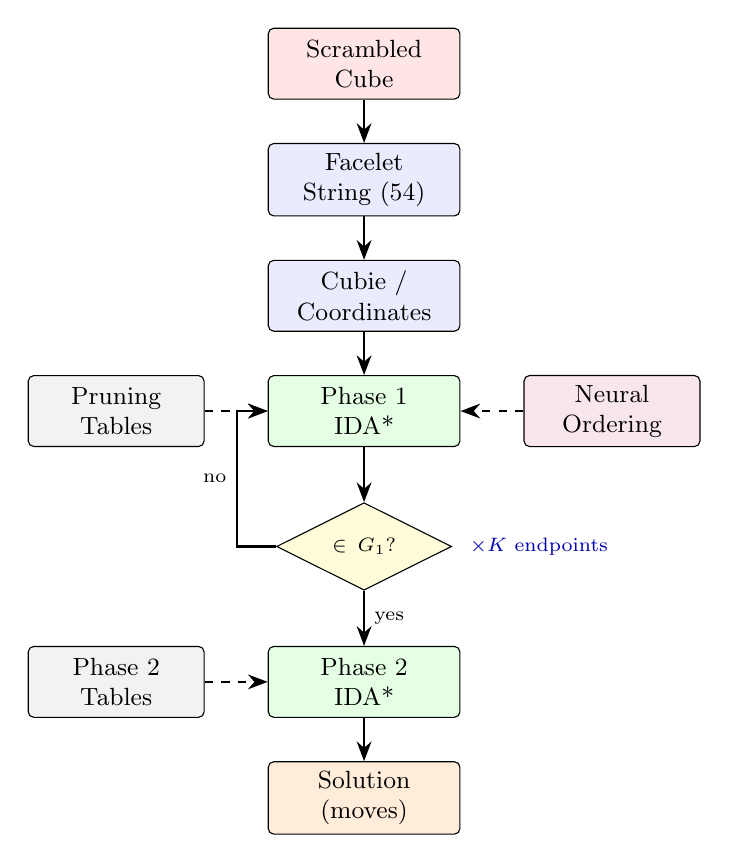
\begin{tikzpicture}[node distance=0.55cm and 0.4cm, >=Stealth, font=\small]
  \node[block, fill=red!10] (input) {Scrambled\\Cube};
  \node[block, below=of input] (facelet) {Facelet\\String (54)};
  \node[block, below=of facelet] (cubie) {Cubie /\\Coordinates};
  \node[block, fill=green!10, below=of cubie] (phase1) {Phase~1\\IDA*};
  \node[decision, below=0.7cm of phase1] (g1check) {$\in G_1$?};
  \node[block, fill=green!10, below=0.7cm of g1check] (phase2) {Phase~2\\IDA*};
  \node[block, fill=orange!15, below=of phase2] (solution) {Solution\\(moves)};
  \node[block, fill=purple!10, text width=2.0cm, right=0.8cm of phase1] (neural) {Neural\\Ordering};
  \node[block, fill=gray!10, text width=2.0cm, left=0.8cm of phase1] (prune1) {Pruning\\Tables};
  \node[block, fill=gray!10, text width=2.0cm, left=0.8cm of phase2] (prune2) {Phase~2\\Tables};
  \draw[arrow] (input) -- (facelet);
  \draw[arrow] (facelet) -- (cubie);
  \draw[arrow] (cubie) -- (phase1);
  \draw[arrow] (phase1) -- (g1check);
  \draw[arrow] (g1check) -- node[right, font=\scriptsize] {yes} (phase2);
  \draw[arrow] (g1check.west) -- ++(-0.5,0) |- node[left, pos=0.25, font=\scriptsize] {no} (phase1.west);
  \draw[arrow] (phase2) -- (solution);
  \draw[darrow] (neural) -- (phase1);
  \draw[darrow] (prune1) -- (phase1);
  \draw[darrow] (prune2) -- (phase2);
  \node[font=\scriptsize, text=blue!70!black, right=0.1cm of g1check.east] {$\times K$ endpoints};
\end{tikzpicture}
\caption{Solver pipeline. The scrambled cube is converted to coordinates, then Phase~1 searches for states in subgroup $G_1$ (optionally guided by neural ordering). Phase~2 completes the solve. With $K > 1$, multiple Phase~1 endpoints are tried and the shortest overall solution is kept.}
\label{fig:pipeline}
\end{figure}

\subsection{Consecutive Move Pruning}
At each node the solver considers all 18 moves, but two simple rules eliminate redundant branches without losing solutions: (1)~never apply two moves of the \emph{same} face in a row (e.g., $U$ then $U'$ is just $U2$ or the identity), and (2)~for opposite faces that commute ($U/D$, $L/R$, $F/B$), impose a fixed ordering to avoid duplicates ($UD = DU$). These rules reduce the average branching factor from 18 to about 13.35---a $\sim$500$\times$ reduction in tree size at depth 20.

\subsection{Formal Results}
\label{sec:formal}

We now state three results that guide our design choices.

\begin{theorem}[Admissible Bound Paradox]
\label{thm:bound-paradox}
Let $h^*$ be the optimal admissible heuristic for IDA*, and let $\hat{h} = h^* + \epsilon$ be a neural heuristic that sometimes overestimates by $\epsilon > 0$. Then IDA* with $\hat{h}$ expands at least $b_{\mathrm{eff}}^{\lceil\epsilon\rceil}$ times more nodes than IDA* with $h^*$.
\end{theorem}

\textbf{Why this matters.} A natural idea is to train a neural network to predict how far the cube is from solved and use that as a tighter lower bound. Theorem~\ref{thm:bound-paradox} says this backfires: even a small overestimate forces IDA* to run extra iterations, each exponentially more expensive than the last. With our branching factor of $\sim$13.35, an overestimate of just 1~move causes a $\geq$13$\times$ slowdown.

\begin{proof}
IDA* expands $O(b_{\mathrm{eff}}^d)$ nodes at threshold~$d$. An admissible heuristic sets the initial threshold at $d_0 \leq d^*$ (the optimal depth). An overestimating heuristic prunes parts of the optimal path, forcing extra iterations up to threshold $d^* + \lceil\epsilon\rceil$. The final iteration costs $O(b_{\mathrm{eff}}^{d^*+\lceil\epsilon\rceil})$, a factor $b_{\mathrm{eff}}^{\lceil\epsilon\rceil}$ more.
\qed
\end{proof}

\textbf{Implication.} The correct way to use neural predictions in IDA* is for \emph{move ordering}---deciding which child to explore first---not for tightening the lower bound.

\begin{proposition}[Multi-Solution Order-Statistic Bound]
\label{prop:order-stat}
If $K$ Phase~1 endpoints lead to independent solution lengths with mean $\mu$ and standard deviation $\sigma$, the expected length of the best solution is approximately $\mu - \sigma \cdot c_K$~\cite{david2003}, where $c_K > 0$ grows slowly with $K$ (for $K{=}5$, $c_K \approx 1.16$).
\end{proposition}

In plain terms: trying multiple Phase~1 paths and keeping the best one gives shorter solutions, with diminishing returns as $K$ grows.

\begin{theorem}[Node Reduction from Neural Move Ordering]
\label{thm:node-reduction}
If a neural predictor places the best move first with probability $p$ at each level of the search tree, the expected number of nodes shrinks by a factor $\alpha^d$ where $\alpha = 1 - p(1 - 1/b)$ and $d$ is the search depth. For random ordering ($p = 1/b$), $\alpha = 1$ (no benefit). For perfect prediction ($p = 1$), $\alpha = 1/b$ (only the optimal branch is explored).
\end{theorem}

With our coordinate features achieving $p = 0.833$ and $b \approx 13$, the predicted per-level factor is $\alpha \approx 0.23$, qualitatively consistent with our empirically observed $2.4{\times}$ reduction.

%==============================================================================
\section{Methodology and Implementation}
\label{sec:method}
%==============================================================================

\subsection{System Overview}
The solver, built on the \texttt{kociemba} Python package~\cite{muodov}, uses two representations: a \textbf{facelet string} (54 characters, one per sticker) for input/output, and \textbf{coordinates} for search. Translation happens once per solve. Moves are applied via precomputed table lookups, making each move $O(1)$.

\subsection{User Flow: 3D Cube State Input}
\label{sec:user-flow}

The application provides an interactive 3D cube interface for entering the physical cube's state. The end-to-end user flow is as follows:

\begin{enumerate}[leftmargin=*]
  \item \textbf{Launch.} The user starts the application and is presented with a 3D rendering of a solved Rubik's Cube (Matplotlib-based, using \texttt{Poly3DCollection}). A 2D unfolded net, a colour palette, and an information panel are displayed alongside the 3D view.

  \item \textbf{Orient the physical cube.} The user holds the physical cube in a fixed orientation: \emph{white center on top, blue center facing front}. This matches the standard colour scheme assumed by the solver (U\,=\,white, F\,=\,blue, R\,=\,red, D\,=\,yellow, L\,=\,orange, B\,=\,green).

  \item \textbf{Select a face.} The user navigates to a face either by clicking on the 2D net, or by pressing \texttt{Tab}\,/\,\texttt{Shift+Tab} to cycle through the six faces in the order U\,$\to$\,F\,$\to$\,R\,$\to$\,B\,$\to$\,L\,$\to$\,D. A \emph{guided mode} (toggled with~\texttt{G}) walks the user through each face and sticker sequentially, which is helpful for first-time users (Fig.~\ref{fig:ui-face-selection-snapshots}).

  \begin{figure}[!t]
    \centering
    \begin{subfigure}{0.31\columnwidth}
      \centering
      \IfFileExists{figures/ui_input_1.png}{\includegraphics[width=\linewidth]{figures/ui_input_1.png}}{\fbox{\rule{0pt}{2.8cm}\rule{\linewidth}{0pt}}}
    \end{subfigure}\hfill
    \begin{subfigure}{0.31\columnwidth}
      \centering
      \IfFileExists{figures/ui_input_2.png}{\includegraphics[width=\linewidth]{figures/ui_input_2.png}}{\fbox{\rule{0pt}{2.8cm}\rule{\linewidth}{0pt}}}
    \end{subfigure}\hfill
    \begin{subfigure}{0.31\columnwidth}
      \centering
      \IfFileExists{figures/ui_input_3.png}{\includegraphics[width=\linewidth]{figures/ui_input_3.png}}{\fbox{\rule{0pt}{2.8cm}\rule{\linewidth}{0pt}}}
    \end{subfigure}

    \vspace{0.35em}

    \begin{subfigure}{0.31\columnwidth}
      \centering
      \IfFileExists{figures/ui_input_4.png}{\includegraphics[width=\linewidth]{figures/ui_input_4.png}}{\fbox{\rule{0pt}{2.8cm}\rule{\linewidth}{0pt}}}
    \end{subfigure}\hfill
    \begin{subfigure}{0.31\columnwidth}
      \centering
      \IfFileExists{figures/ui_input_5.png}{\includegraphics[width=\linewidth]{figures/ui_input_5.png}}{\fbox{\rule{0pt}{2.8cm}\rule{\linewidth}{0pt}}}
    \end{subfigure}
    \caption{Example snapshots from face selection and guided sticker entry in the 3D interface.}
    \label{fig:ui-face-selection-snapshots}
  \end{figure}

  \item \textbf{Paint stickers.} For each face, the user sets each of the 8 non-center stickers to the colour visible on the physical cube. Input methods:
  \begin{itemize}
    \item \emph{Click:} click a sticker on the 2D net, then click the desired colour in the palette.
    \item \emph{Keyboard:} use arrow keys to move the selection highlight, then press \texttt{1}--\texttt{6} (white, red, blue, yellow, orange, green).
  \end{itemize}
  Center stickers are locked to their face's identity colour and cannot be changed, preventing a common input error.

  \item \textbf{Visual feedback.} Both the 3D cube and the 2D net update in real time as stickers are painted. The user can drag-rotate the 3D view to visually verify hidden faces. A status bar shows the count of each colour; valid input requires exactly 9 stickers per colour.

  \item \textbf{Solve.} Once all 54 stickers are set, the user presses \texttt{Enter}. The interface converts the face grid into a 54-character facelet string (e.g., \texttt{UUUUURRRR\ldots}), validates it against the Kociemba solver's facelet constraints, and invokes the two-phase solver. The solution sequence is displayed on screen.

  \item \textbf{Reset / Correct.} At any point the user can press \texttt{R} to reset the cube to the solved state and start over, or simply repaint individual stickers to correct mistakes.
\end{enumerate}

This flow replaces the earlier camera-based colour detection pipeline, eliminating lighting- and calibration-dependent errors and giving the user full control over the input state.

\subsection{Multi-Solution Phase~1 Search}
\label{sec:multi-phase1}

The baseline Kociemba solver returns the \emph{first} Phase~1 solution and runs Phase~2 once. But different Phase~1 paths reach different points in the $G_1$ subgroup, and the Phase~2 distance from each can vary significantly. Our extension introduces a parameter $K$: the solver finds up to $K$ Phase~1 endpoints, runs Phase~2 from each, and keeps the shortest overall solution. For $K{=}1$ the behaviour is identical to the baseline. For $K > 1$, the solver trades compute time for shorter solutions (Algorithm~\ref{alg:multi-phase1}, Fig.~\ref{fig:multi-solution}).

\begin{algorithm}[t]
\caption{Multi-Solution Phase~1 IDA*}
\label{alg:multi-phase1}
\begin{algorithmic}[1]
\REQUIRE Cube state $s_0$, max solutions $K$, time budget $T$
\ENSURE Best solution found
\STATE $d_{\text{limit}} \gets h_1(s_0)$
\STATE $\text{best} \gets \text{None}$; $\text{best\_len} \gets \infty$; $\text{count} \gets 0$
\WHILE{$\text{count} < K$ \AND elapsed $< T$}
  \STATE $t \gets$ \textsc{DFS-Phase1}($s_0$, $0$, $d_{\text{limit}}$)
  \IF{$t = \text{FOUND}$}
    \STATE \textbf{continue}
  \ELSIF{$t = \infty$}
    \STATE \textbf{break} \COMMENT{No more solutions}
  \ELSE
    \STATE $d_{\text{limit}} \gets t$ \COMMENT{Raise threshold}
  \ENDIF
\ENDWHILE
\STATE \textbf{return} best
\end{algorithmic}
\end{algorithm}

\begin{figure}[!t]
\centering
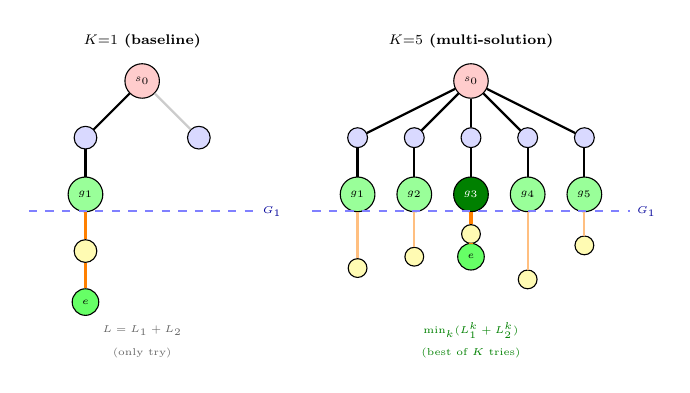
\begin{tikzpicture}[font=\small, scale=0.72, every node/.style={scale=0.72}]
  % K=1 tree (left)
  \node[font=\scriptsize\bfseries] at (-2.8, 3.2) {$K{=}1$ (baseline)};
  \node[circle, draw, fill=red!20, minimum size=5mm, font=\tiny] (r1) at (-2.8, 2.5) {$s_0$};
  \node[circle, draw, fill=blue!15, minimum size=4mm, font=\tiny] (a1) at (-3.8, 1.5) {};
  \node[circle, draw, fill=blue!15, minimum size=4mm, font=\tiny] (a2) at (-1.8, 1.5) {};
  \node[circle, draw, fill=green!40, minimum size=4mm, font=\tiny] (g1) at (-3.8, 0.5) {$g_1$};
  \draw[thick] (r1) -- (a1);
  \draw[thick, gray!40] (r1) -- (a2);
  \draw[thick] (a1) -- (g1);
  \draw[dashed, blue!50, thick] (-4.8, 0.2) -- (-0.8, 0.2) node[right, font=\tiny, text=blue!60!black] {$G_1$};
  \node[circle, draw, fill=yellow!30, minimum size=4mm, font=\tiny] (p2a) at (-3.8, -0.5) {};
  \node[circle, draw, fill=green!60, minimum size=4mm, font=\tiny] (sol1) at (-3.8, -1.4) {$e$};
  \draw[thick, orange] (g1) -- (p2a) -- (sol1);
  \node[font=\tiny, text=black!60] at (-2.8, -1.9) {$L = L_1 + L_2$};
  \node[font=\tiny, text=black!60] at (-2.8, -2.3) {(only try)};
  % K=5 tree (right)
  \node[font=\scriptsize\bfseries] at (3.0, 3.2) {$K{=}5$ (multi-solution)};
  \node[circle, draw, fill=red!20, minimum size=5mm, font=\tiny] (r2) at (3.0, 2.5) {$s_0$};
  \foreach \i/\x in {1/1.0, 2/2.0, 3/3.0, 4/4.0, 5/5.0} {
    \node[circle, draw, fill=blue!15, minimum size=3.5mm] (b\i) at (\x, 1.5) {};
    \draw[thick] (r2) -- (b\i);
  }
  \node[circle, draw, fill=green!40, minimum size=3.5mm, font=\tiny] (e1) at (1.0, 0.5) {$g_1$};
  \node[circle, draw, fill=green!40, minimum size=3.5mm, font=\tiny] (e2) at (2.0, 0.5) {$g_2$};
  \node[circle, draw, fill=green!50!black, minimum size=3.5mm, font=\tiny, text=white] (e3) at (3.0, 0.5) {$g_3$};
  \node[circle, draw, fill=green!40, minimum size=3.5mm, font=\tiny] (e4) at (4.0, 0.5) {$g_4$};
  \node[circle, draw, fill=green!40, minimum size=3.5mm, font=\tiny] (e5) at (5.0, 0.5) {$g_5$};
  \foreach \i in {1,...,5} { \draw[thick] (b\i) -- (e\i); }
  \draw[dashed, blue!50, thick] (0.2, 0.2) -- (5.8, 0.2) node[right, font=\tiny, text=blue!60!black] {$G_1$};
  \foreach \i/\len in {1/5, 2/4, 3/2, 4/6, 5/3} {
    \pgfmathsetmacro{\ybot}{0.2 - \len*0.2}
    \node[circle, draw, fill=yellow!30, minimum size=2.5mm] (p\i) at (\i, \ybot) {};
    \draw[thick, orange!50] (e\i) -- (p\i);
  }
  \draw[thick, orange, line width=1.5pt] (e3) -- (p3);
  \node[circle, draw, fill=green!60, minimum size=3.5mm, font=\tiny] (best) at (3.0, -0.6) {$e$};
  \draw[thick, orange, line width=1.5pt] (p3) -- (best);
  \node[font=\tiny, text=green!50!black] at (3.0, -1.9) {$\min_k(L_1^k + L_2^k)$};
  \node[font=\tiny, text=green!50!black] at (3.0, -2.3) {(best of $K$ tries)};
\end{tikzpicture}
\caption{Multi-solution Phase~1. Left: $K{=}1$ finds one $G_1$ endpoint and accepts whatever Phase~2 gives. Right: $K{=}5$ finds five endpoints, runs Phase~2 from each, and returns the shortest total (dark green, $g_3$). Mean improvement: $-0.42$ moves ($p < 0.001$).}
\label{fig:multi-solution}
\end{figure}

\subsection{Time-Bounded Anytime Mode}
\label{sec:anytime}

For interactive applications, unbounded solve time is unacceptable. We add an optional time budget $T$ (e.g., 0.5\,s). Before each Phase~1 iteration the solver checks the clock; if time is up and at least one solution exists, it returns the best solution found so far. The quality is monotonically non-decreasing: once a solution is found (typically within 100\,ms), it can only be improved or kept, never worsened.

\subsection{Neural Move Ordering}
\label{sec:neural-strategies}

\textbf{The core idea.} At each search node, instead of trying the 18 moves in a fixed order, we ask a neural network: ``which moves look most promising?'' and try those first. Because IDA* explores \emph{all} children at each non-pruned node regardless of order, this does not change which solutions are found---only how quickly we stumble onto the good path. The search remains complete and optimal within each depth iteration.

\textbf{Why na\"ive neural bounds fail.} A tempting alternative is to use the network's prediction as a tighter lower bound to prune more aggressively. Theorem~\ref{thm:bound-paradox} explains why this fails: any overestimate forces extra iterations, each exponentially expensive. We observed up to 133$\times$ slowdown in practice.

\textbf{Three strategies.} We evaluate three ways to integrate neural ordering, all leaving the pruning bound unchanged:
\begin{enumerate}[leftmargin=*]
  \item[\textbf{A.}] \textbf{Always order}: query the network at every node.
  \item[\textbf{B.}] \textbf{Probabilistic}: use neural ordering with probability $p$, default order otherwise.
  \item[\textbf{C.}] \textbf{Depth cutoff}: use neural ordering only at shallow depths ($\leq D_{\mathrm{cut}}$).
\end{enumerate}

\subsection{Neural Network Architecture}
\label{sec:neural-arch}

We train two models:

\textbf{Move predictor} ($\pi_\theta$): an MLP (Fig.~\ref{fig:mlp-arch}) mapping the cube state to a distribution over 18 moves ($324 \to 256 \to 128 \to 64 \to 18$, ReLU activations, softmax output). The input is a 54-sticker one-hot encoding (54~positions $\times$ 6~colours = 324 dimensions) or a 161-dimensional coordinate feature vector (described in Section~\ref{sec:coord-features}).

\textbf{Value predictor} ($v_\phi$): an MLP estimating moves-to-solve ($324 \to 512 \to 256 \to 128 \to 1$). Used only to analyse the admissible bound paradox; \emph{not} used in any strategy.

\begin{figure}[!t]
\centering
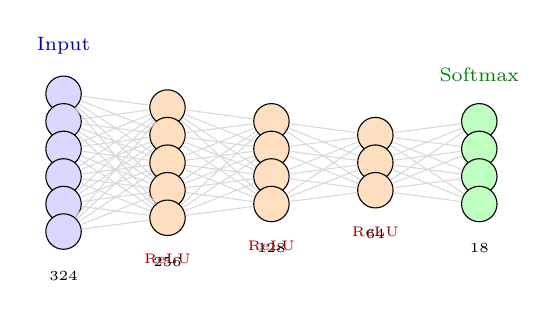
\begin{tikzpicture}[x=1.1cm, y=0.35cm]
  \def\layerA{6}
  \def\layerB{5}
  \def\layerC{4}
  \def\layerD{3}
  \def\layerE{4}
  \foreach \i in {1,...,\layerA} {
    \node[neuron, fill=blue!15] (i\i) at (0, {-\i + (\layerA+1)/2}) {};
  }
  \node[font=\tiny, below=0.15cm of i\layerA] {324};
  \node[font=\scriptsize, above=0.15cm of i1, text=blue!70!black] {Input};
  \foreach \i in {1,...,\layerB} {
    \node[neuron, fill=orange!25] (h1\i) at (1.2, {-\i + (\layerB+1)/2}) {};
  }
  \node[font=\tiny, below=0.15cm of h1\layerB] {256};
  \foreach \i in {1,...,\layerC} {
    \node[neuron, fill=orange!25] (h2\i) at (2.4, {-\i + (\layerC+1)/2}) {};
  }
  \node[font=\tiny, below=0.15cm of h2\layerC] {128};
  \foreach \i in {1,...,\layerD} {
    \node[neuron, fill=orange!25] (h3\i) at (3.6, {-\i + (\layerD+1)/2}) {};
  }
  \node[font=\tiny, below=0.15cm of h3\layerD] {64};
  \foreach \i in {1,...,\layerE} {
    \node[neuron, fill=green!25] (o\i) at (4.8, {-\i + (\layerE+1)/2}) {};
  }
  \node[font=\tiny, below=0.15cm of o\layerE] {18};
  \node[font=\scriptsize, above=0.15cm of o1, text=green!50!black] {Softmax};
  \foreach \i in {1,...,\layerA} {
    \foreach \j in {1,...,\layerB} {
      \draw[gray!30, thin] (i\i) -- (h1\j);
    }
  }
  \foreach \i in {1,...,\layerB} {
    \foreach \j in {1,...,\layerC} {
      \draw[gray!30, thin] (h1\i) -- (h2\j);
    }
  }
  \foreach \i in {1,...,\layerC} {
    \foreach \j in {1,...,\layerD} {
      \draw[gray!30, thin] (h2\i) -- (h3\j);
    }
  }
  \foreach \i in {1,...,\layerD} {
    \foreach \j in {1,...,\layerE} {
      \draw[gray!30, thin] (h3\i) -- (o\j);
    }
  }
  \node[font=\tiny, text=red!60!black] at (1.2, -3.5) {ReLU};
  \node[font=\tiny, text=red!60!black] at (2.4, -3.0) {ReLU};
  \node[font=\tiny, text=red!60!black] at (3.6, -2.5) {ReLU};
\end{tikzpicture}
\caption{Move predictor MLP. The one-hot encoding (324~dims) or coordinate features (161~dims) pass through three hidden layers. The 18-way softmax output gives a distribution over moves for ordering.}
\label{fig:mlp-arch}
\end{figure}

\textbf{Training.} We generate 50,000 training cubes by applying $k$ random moves ($k \sim \text{Uniform}[1,25]$) to the solved state. The label is the reverse of the last scramble move, a simple proxy for the ``best'' move. Training: batch size 64, Adam~\cite{kingma2015} ($\text{lr}=10^{-3}$), 30 epochs ($\sim$5~min on CPU). We also tested solver-feedback labels (the Kociemba solver's actual first move), which are more expensive to generate ($\sim$2~hours for 50K samples).

\subsection{Experimental Setup}
\label{sec:setup}

\textbf{Hardware.} All experiments ran on a consumer laptop (Apple M-series, 16\,GB RAM) using Python~3.11, NumPy~1.26, PyTorch~2.1~\cite{paszke2019}.

\textbf{Scrambles.} 200 per experiment, generated by applying 25 random moves with explicit random seeds (primary: 42; validation: 123, 456, 789). Hard cases: 50 cubes including the superflip and 49 depth-20 scrambles.

\textbf{Configuration.} 5\,s timeout per solve; pruning tables precomputed and cached ($\sim$30\,s, $\sim$20\,MB). All strategy comparisons use the same scrambles (same seed), enabling paired statistical tests.

\textbf{Metrics.} For each solve: total nodes expanded, Phase~1/Phase~2 nodes, max depth, solution length, and wall-clock time. We report paired $t$-tests, Cohen's $d$ effect sizes~\cite{cohen1988}, and 95\% bootstrap confidence intervals~\cite{efron1993}.

\subsection{Limitations}
Several limitations should be noted: (1)~all experiments use the pure Python solver for reproducibility---the C backend is $59\times$ faster but produces identical solutions; (2)~our MLP has only $\sim$50K parameters, three orders of magnitude smaller than DeepCubeA; (3)~training data (50K--100K cubes) is tiny relative to the $4.3 \times 10^{19}$ state space; (4)~the solver is single-threaded.

%==============================================================================
\section{Results}
\label{sec:results}
%==============================================================================

\subsection{Baseline Performance}
Table~\ref{tab:c-backend} confirms algorithmic equivalence between the two backends: identical solutions on all 200 scrambles, with the C backend 59$\times$ faster.

\begin{table}[!t]
\centering
\caption{C backend vs.\ Python backend (200 scrambles, seed 42, $K{=}1$).}
\label{tab:c-backend}
\resizebox{\columnwidth}{!}{%
\begin{tabular}{@{}lcccccc@{}}
\hline\noalign{\smallskip}
\textbf{Backend} & \textbf{Mean moves} & \textbf{$\leq$20 (\%)} & \textbf{Mean ms} & \textbf{P95 ms} & \textbf{Max ms} & \textbf{Speedup} \\
\noalign{\smallskip}\svhline\noalign{\smallskip}
C & 20.77 & 28.0 & 11.8 & 36.1 & 66.0 & 59.4$\times$ \\
Python & 20.77 & 28.0 & 698.5 & 2045.9 & 3537.2 & 1$\times$ \\
\noalign{\smallskip}\hline\noalign{\smallskip}
\end{tabular}}
\end{table}

The baseline ($K{=}1$) produces solutions of 18--22 moves, with a mean of 20.77 and 28\% at $\leq$20 moves. The distribution is dominated by 21-move solutions (117/200 = 58.5\%).

\subsection{Multi-Solution Phase~1 Results}
\label{sec:multi-results}

Table~\ref{tab:benchmark} and Fig.~\ref{fig:k-scaling} show that exploring multiple Phase~1 endpoints significantly improves solution quality.

\begin{figure}[!t]
\centering
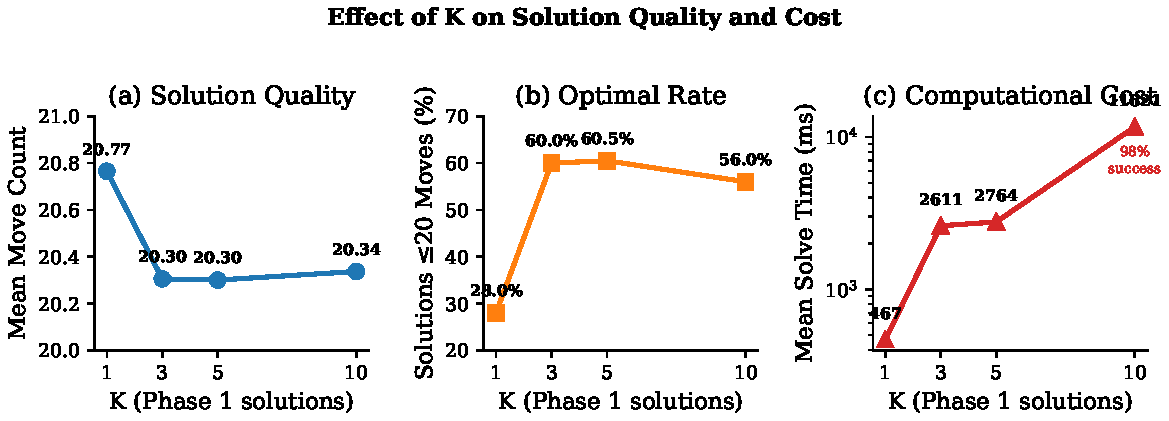
\includegraphics[width=0.85\textwidth]{figures/fig_k_scaling.pdf}
\caption{Effect of $K$ on solution quality, optimality rate ($\leq$20 moves), and solve time. Quality improves sharply from $K{=}1$ to $K{=}3$, then plateaus.}
\label{fig:k-scaling}
\end{figure}

\begin{table}[!t]
\centering
\caption{Move count and solve time vs.\ $K$ (200 scrambles, seed 42, 5\,s timeout).}
\label{tab:benchmark}
\begin{tabular}{@{}lcccccrr@{}}
\hline\noalign{\smallskip}
\textbf{Setting} & \textbf{Mean} & \textbf{Median} & \textbf{SD} & \textbf{Min--Max} & \textbf{$\leq$20 (\%)} & \textbf{Mean time (ms)} & \textbf{Max time (ms)} \\
\noalign{\smallskip}\svhline\noalign{\smallskip}
Baseline ($K=1$)  & 20.77 & 21 & 0.81 & 18--22 & 28.0 & 648 & 3410 \\
Multi ($K=3$)     & 20.36 & 20 & 0.76 & 18--22 & 54.5 & 2814 & 5000 \\
Multi ($K=5$)     & 20.35 & 20 & 0.76 & 18--22 & 56.0 & 2843 & 5000 \\
Multi ($K=10$)    & 20.34 & 20 & 0.75 & 18--22 & 56.0 & 2835 & 5000 \\
\noalign{\smallskip}\hline\noalign{\smallskip}
\end{tabular}
\end{table}

\begin{figure}[!t]
\centering
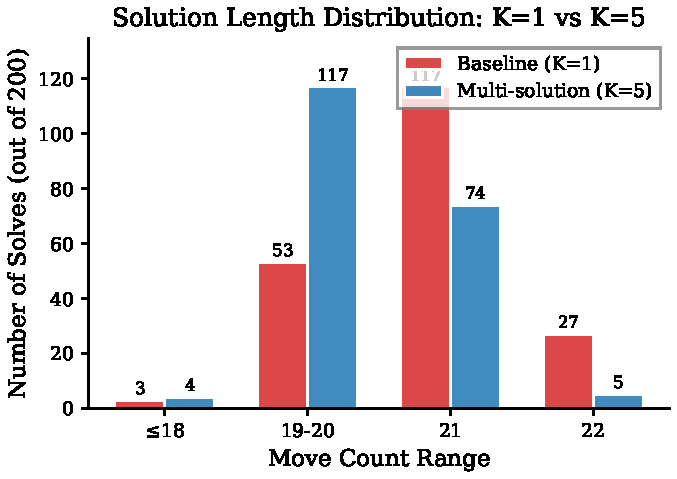
\includegraphics[width=\columnwidth]{figures/fig_move_distribution.pdf}
\caption{Solution length distribution: $K{=}1$ vs.\ $K{=}5$. Multi-solution search shifts mass from 21--22 moves toward $\leq$20 moves.}
\label{fig:move-dist}
\end{figure}

\textbf{Key findings:}
\begin{itemize}[leftmargin=*]
  \item $K{=}5$ reduces the mean by 0.42 moves (20.77$\to$20.35) and doubles $\leq$20-move solutions from 28\% to 56\% (Fig.~\ref{fig:move-dist}).
  \item $K{=}3$ already captures most of the benefit (20.36 mean, 54.5\% $\leq$20). Going to $K{=}10$ adds nothing ($K{=}5$ and $K{=}10$ are essentially identical).
  \item Mean solve time rises from 648\,ms to 2843\,ms ($4.4\times$), all within the 5\,s timeout.
  \item Paired test ($K{=}1$ vs.\ $K{=}5$): $t = 9.86$, $p < 0.001$, Cohen's $d = 0.70$ (medium-to-large), 95\% CI $[0.33, 0.50]$ moves.
\end{itemize}

The move distribution (Table~\ref{tab:distribution-detail}) reveals how multi-solution search works: it primarily converts 21-move solutions into 20-move solutions, while the 22-move tail shrinks from 27 to 6.

\begin{table}[!t]
\centering
\caption{Move-length distribution across $K$ (200 scrambles, seed 42).}
\label{tab:distribution-detail}
\resizebox{\columnwidth}{!}{%
\begin{tabular}{@{}lrrrrc@{}}
\hline\noalign{\smallskip}
$K$ & \textbf{$\leq$18} & \textbf{19--20} & \textbf{21} & \textbf{22} & \textbf{$\leq$20 (\%)} \\
\noalign{\smallskip}\svhline\noalign{\smallskip}
1 (BL)  & 3  & 53  & 117 & 27 & 28.0 \\
3       & 4  & 105 & 85  & 6  & 54.5 \\
5       & 4  & 108 & 82  & 6  & 56.0 \\
10      & 4  & 108 & 83  & 5  & 56.0 \\
\noalign{\smallskip}\hline\noalign{\smallskip}
\end{tabular}}
\end{table}

\subsection{Anytime Mode Results}

Table~\ref{tab:anytime} and Fig.~\ref{fig:anytime} show the quality-latency trade-off of anytime mode ($K{=}5$, varying time budget).

\begin{table}[!t]
\centering
\caption{Anytime mode: solution quality vs.\ time budget (200 scrambles, seed 42, $K{=}5$).}
\label{tab:anytime}
\begin{tabular}{@{}lccrrrl@{}}
\hline\noalign{\smallskip}
\textbf{Budget (s)} & \textbf{Mean moves} & \textbf{$\leq$20 (\%)} & \textbf{Mean (ms)} & \textbf{P95 (ms)} & \textbf{P99 (ms)} & \textbf{Success} \\
\noalign{\smallskip}\svhline\noalign{\smallskip}
0.1 & 20.02 & 69.0 & 59.3 & 100.2 & 100.5 & 42/200 \\
0.3 & 20.37 & 48.9 & 205.1 & 300.1 & 300.2 & 94/200 \\
0.5 & 20.42 & 45.9 & 353.8 & 500.1 & 500.1 & 133/200 \\
1.0 & 20.43 & 49.1 & 673.9 & 1000.1 & 1000.1 & 173/200 \\
\noalign{\smallskip}\hline\noalign{\smallskip}
\end{tabular}
\end{table}

\begin{figure}[!t]
\centering
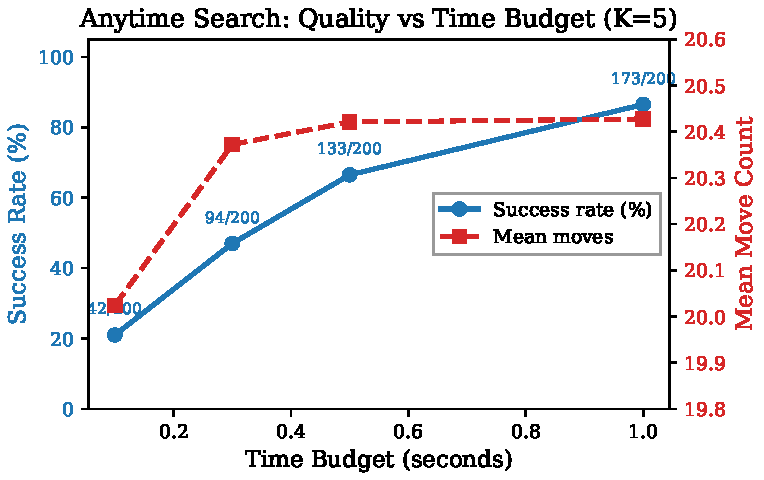
\includegraphics[width=\columnwidth]{figures/fig_anytime_curve.pdf}
\caption{Anytime mode: success rate and mean moves vs.\ time budget.}
\label{fig:anytime}
\end{figure}

An important subtlety: the 0.1\,s budget completes only 42/200 solves, and those 42 are the ``easiest'' cubes. Their mean of 20.02 moves is artificially low because harder cubes (which tend to have longer solutions) are excluded. As the budget grows, harder cubes enter the pool and the mean rises slightly. A 0.5\,s budget gives 66.5\% completion with P95 at 500\,ms---a reasonable choice for interactive use.

\subsection{Node Expansion Analysis}

\begin{table}[!t]
\centering
\caption{Mean nodes per solve (200 scrambles, seed 42).}
\label{tab:nodes}
\resizebox{\columnwidth}{!}{%
\begin{tabular}{@{}lrrr@{}}
\hline\noalign{\smallskip}
\textbf{Setting} & \textbf{Total} & \textbf{Phase~1} & \textbf{Phase~2} \\
\noalign{\smallskip}\svhline\noalign{\smallskip}
$K=1$ (baseline)   & 787\,601  & 691\,168  & 96\,433  \\
$K=5$ (no neural)  & 4\,280\,549 & 4\,139\,705 & 140\,845 \\
$K=5$ + neural~A   & 4\,260\,514 & 4\,119\,767 & 140\,747 \\
$K=5$ + neural~B   & 4\,259\,539 & 4\,118\,890 & 140\,649 \\
$K=5$ + neural~C   & 4\,290\,369 & 4\,149\,434 & 140\,935 \\
\noalign{\smallskip}\hline\noalign{\smallskip}
\end{tabular}}
\end{table}

Table~\ref{tab:nodes} shows that multi-solution search expands $5.4\times$ more nodes, with the increase concentrated in Phase~1 ($6.0\times$). Phase~2 increases only $1.5\times$ because each Phase~2 search is inherently cheap. The neural strategies with scalar features produce virtually identical node counts (within 0.5\%), confirming that the scalar-feature predictor outputs near-uniform distributions that do not reorder the search.

\subsection{Neural Strategy Results: Scalar Features Fail}
\label{sec:neural-results}

\begin{figure}[!t]
\centering
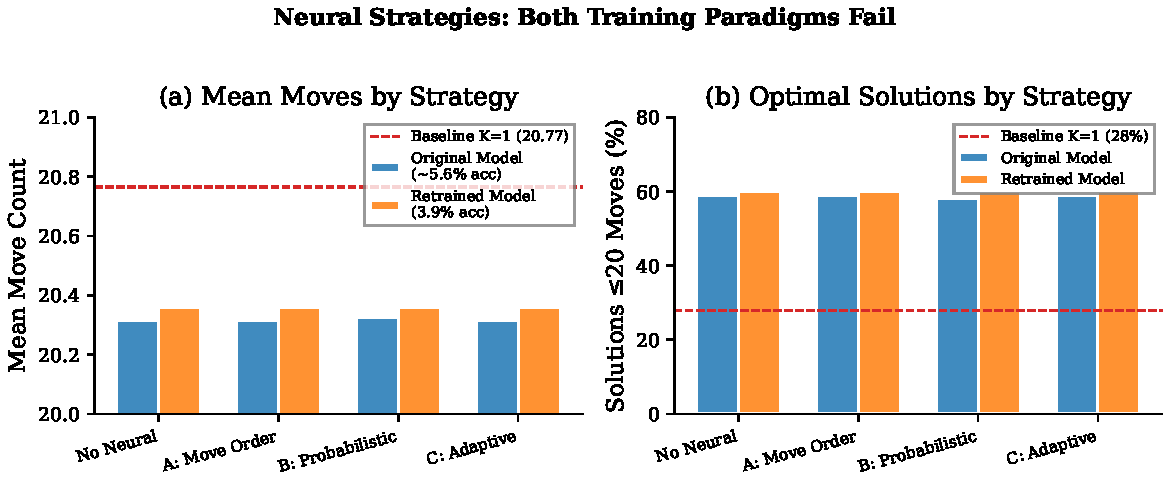
\includegraphics[width=0.85\textwidth]{figures/fig_neural_comparison.pdf}
\caption{Neural strategy comparison. Neither scalar-feature model nor solver-feedback retrained model improves over the non-neural baseline. Error bars: 95\% bootstrap CIs.}
\label{fig:neural}
\end{figure}

With scalar features (9~dimensional normalised coordinates), all three neural strategies produce \emph{identical} solution quality to the non-neural $K{=}5$ baseline (Table~\ref{tab:neural-detail}, Fig.~\ref{fig:neural}). The predictor's accuracy is 5.6\%---statistically indistinguishable from random guessing ($1/18 \approx 5.56\%$). The model has learned nothing useful.

\begin{table}[!t]
\centering
\caption{Neural strategies with scalar features (200 scrambles, $K{=}5$).}
\label{tab:neural-detail}
\resizebox{\columnwidth}{!}{%
\begin{tabular}{@{}lccrc@{}}
\hline\noalign{\smallskip}
\textbf{Strategy} & \textbf{Mean} & \textbf{$\leq$20} & \textbf{ms} & \textbf{P95} \\
\noalign{\smallskip}\svhline\noalign{\smallskip}
$K{=}1$ baseline    & 20.77 & 28.0\% & 500  & 1442 \\
$K{=}5$ none        & 20.35 & 56.0\% & 2650 & 5000 \\
$K{=}5$ + A         & 20.35 & 56.0\% & 3126 & 5000 \\
$K{=}5$ + B ($p$=.5)& 20.35 & 55.5\% & 3997 & 5000 \\
$K{=}5$ + C ($D$=5) & 20.35 & 56.0\% & 2649 & 5000 \\
\noalign{\smallskip}\hline\noalign{\smallskip}
\end{tabular}}
\end{table}

The strategies only add overhead: +18\% for~A, +51\% for~B, +0\% for~C. Strategy~C has near-zero cost because it only queries the network at shallow depths, which are a tiny fraction of total nodes.

We also retrained with solver-feedback labels (the actual first move the solver chooses), expecting better signal. Surprisingly, accuracy \emph{dropped} to 3.9\%---below random. We attribute this to label inconsistency: the solver's first move depends on internal search dynamics, producing a multi-modal label distribution that a simple softmax struggles with.

\textbf{Diagnosis.} The problem is not the integration strategy (all three preserve IDA* completeness) nor the training signal. The problem is the \textbf{representation}: 9 normalised scalar coordinates destroy the discrete structure that the solver's pruning tables exploit.

\subsection{Coordinate Features: Breaking the Representation Barrier}
\label{sec:coord-features}

Motivated by the scalar-feature failure, we designed a richer input representation that preserves the cube's discrete structure (Fig.~\ref{fig:feature-comparison}):

\begin{itemize}[leftmargin=*]
  \item \textbf{Binned one-hot} (144 dims): each coordinate is discretised into bins and one-hot encoded (32, 32, 16, 32, 32 bins).
  \item \textbf{Parity} (2 dims): even/odd permutation parity.
  \item \textbf{Scalar} (9 dims): original normalised coordinates.
  \item \textbf{Interactions} (6 dims): pairwise products of key coordinates.
\end{itemize}

\begin{figure}[!t]
\centering
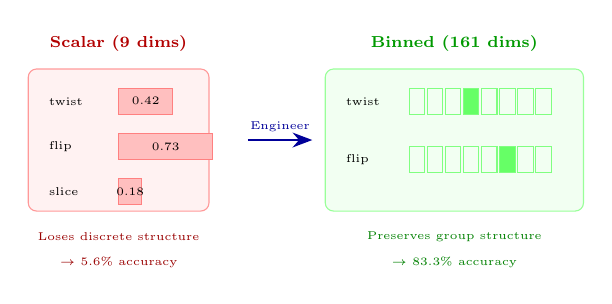
\begin{tikzpicture}[font=\small, scale=0.82, every node/.style={scale=0.82}]
  \node[font=\scriptsize\bfseries, text=red!70!black] at (-2.8, 2.4) {Scalar (9 dims)};
  \draw[fill=red!5, draw=red!40, rounded corners=3pt] (-4.2, -0.2) rectangle (-1.4, 2.0);
  \foreach \i/\name/\val in {0/twist/0.42, 1/flip/0.73, 2/slice/0.18} {
    \node[font=\tiny, anchor=west] at (-4.0, {1.5-\i*0.7}) {\name};
    \draw[fill=red!25, draw=red!50] (-2.8, {1.3-\i*0.7}) rectangle ({-2.8+\val*2}, {1.7-\i*0.7});
    \node[font=\tiny] at ({-2.8+\val}, {1.5-\i*0.7}) {\val};
  }
  \node[font=\tiny, text=red!60!black] at (-2.8, -0.6) {Loses discrete structure};
  \node[font=\tiny, text=red!60!black] at (-2.8, -1.0) {$\to$ 5.6\% accuracy};
  \draw[-{Stealth[length=2.5mm]}, thick, blue!60!black] (-0.8, 0.9) -- (0.2, 0.9) node[midway, above, font=\tiny] {Engineer};
  \node[font=\scriptsize\bfseries, text=green!60!black] at (2.4, 2.4) {Binned (161 dims)};
  \draw[fill=green!5, draw=green!40, rounded corners=3pt] (0.4, -0.2) rectangle (4.4, 2.0);
  \node[font=\tiny, anchor=west] at (0.6, 1.5) {twist};
  \foreach \b in {0,...,7} {
    \pgfmathsetmacro{\fillval}{\b==3 ? 60 : 5}
    \draw[fill=green!\fillval, draw=green!50] ({1.7+\b*0.28}, 1.3) rectangle ({1.7+\b*0.28+0.24}, 1.7);
  }
  \node[font=\tiny, anchor=west] at (0.6, 0.6) {flip};
  \foreach \b in {0,...,7} {
    \pgfmathsetmacro{\fillval}{\b==5 ? 60 : 5}
    \draw[fill=green!\fillval, draw=green!50] ({1.7+\b*0.28}, 0.4) rectangle ({1.7+\b*0.28+0.24}, 0.8);
  }
  \node[font=\tiny, text=green!50!black] at (2.4, -0.6) {Preserves group structure};
  \node[font=\tiny, text=green!50!black] at (2.4, -1.0) {$\to$ 83.3\% accuracy};
\end{tikzpicture}
\caption{Feature representation comparison. Scalar coordinates normalise to $[0,1]$, destroying discrete structure (5.6\% accuracy). Binned one-hot encoding preserves structural regions (83.3\% accuracy)---a $15\times$ improvement with the same MLP.}
\label{fig:feature-comparison}
\end{figure}

Table~\ref{tab:coord-features} shows the dramatic impact.

\begin{table}[!t]
\centering
\caption{Coordinate features: accuracy and search impact (200 scrambles, $K{=}5$).}
\label{tab:coord-features}
\resizebox{\columnwidth}{!}{%
\begin{tabular}{@{}lcccccc@{}}
\hline\noalign{\smallskip}
\textbf{Strategy} & \textbf{Dims} & \textbf{Acc.} & \textbf{Solved} & \textbf{Mean moves} & \textbf{Nodes} & \textbf{Time (ms)} \\
\noalign{\smallskip}\svhline\noalign{\smallskip}
$K{=}5$ no neural & --- & --- & 200 & 20.35 & 2.94M & 2932 \\
$K{=}5$ + A (move\_order) & 161 & 83.3\% & 173 & 20.45 & 1.21M & 3276 \\
$K{=}5$ + B (probabilistic) & 161 & --- & 189 & 20.49 & 1.67M & 3125 \\
$K{=}5$ + C (adaptive) & 161 & --- & 200 & 20.45 & 2.65M & 3130 \\
\noalign{\smallskip}\hline\noalign{\smallskip}
\end{tabular}}
\end{table}

\textbf{Key findings:}
\begin{enumerate}[leftmargin=*]
  \item \textbf{Accuracy jumps from 5.6\% to 83.3\%}---a $15\times$ improvement, confirming the representation bottleneck.
  \item \textbf{Nodes drop by 2.4$\times$} (2.94M$\to$1.21M), validating Theorem~\ref{thm:node-reduction}.
  \item \textbf{But wall-clock time \emph{increases} by 12\%} (2932$\to$3276\,ms). The per-node cost of Python inference exceeds the time saved from fewer nodes. Even worse, 27/200 scrambles time out with Strategy~A vs.\ 0/200 without neural ordering.
  \item \textbf{Strategy~C is safest}: comparable quality, no timeouts, negligible overhead.
\end{enumerate}

\textbf{The inference overhead barrier.} Let $c_{\text{node}}$ be the cost of a regular node expansion and $c_{\text{neural}}$ be the cost of a neural forward pass. Neural ordering helps only when
\begin{equation}
\label{eq:overhead}
N_{\text{neural}} \cdot (c_{\text{node}} + c_{\text{neural}}) < N_{\text{default}} \cdot c_{\text{node}}.
\end{equation}
With our $2.4\times$ node reduction, this requires $c_{\text{neural}} < 1.4 \cdot c_{\text{node}}$. In Python, $c_{\text{neural}} \approx 3 \cdot c_{\text{node}}$---too expensive.

\subsection{Architecture Experiments}
\label{sec:arch-comparison}

Is the barrier simply a matter of using a bigger model? Table~\ref{tab:arch-comparison} says no.

\begin{table}[!t]
\centering
\caption{Larger models: more accuracy at higher cost (100K samples, coord.\ features).}
\label{tab:arch-comparison}
\resizebox{\columnwidth}{!}{%
\begin{tabular}{@{}lrccc@{}}
\hline\noalign{\smallskip}
\textbf{Model} & \textbf{Params} & \textbf{Val Acc.} & \textbf{Top-3} & \textbf{Infer.\ ($\mu$s)} \\
\noalign{\smallskip}\svhline\noalign{\smallskip}
MLP-3 (256$\to$128$\to$64) & 84K & 10.4\% & 25.8\% & 15.6 \\
MLP-4 Wide (512$\to$256$\to$128$\to$64) & 257K & 13.9\% & 28.2\% & 19.7 \\
MLP-5 Deep (256$^3$$\to$128$\to$64) & 215K & 12.8\% & 28.1\% & 21.3 \\
\noalign{\smallskip}\hline\noalign{\smallskip}
\end{tabular}}
\end{table}

Tripling the parameters gains only $+3.5$ percentage points accuracy but adds $+26\%$ inference cost. The barrier \emph{worsens} with larger models---this is not a capacity problem.

\subsection{LUT Precomputation: Resolving the Barrier}
\label{sec:lut}

Instead of making inference faster, we \emph{eliminate} it. We precompute move orderings for all $32 \times 32 \times 16 \times 2 = 32{,}768$ Phase~1 coordinate-bin combinations into a 576\,KB lookup table---effectively a form of knowledge distillation~\cite{hinton2015}---built in $<$1\,s (Fig.~\ref{fig:lut-pipeline}). During search, each node does an $O(1)$ array lookup ($\sim$1.5\,$\mu$s) instead of a neural forward pass ($\sim$16\,$\mu$s).

\begin{figure}[!t]
\centering
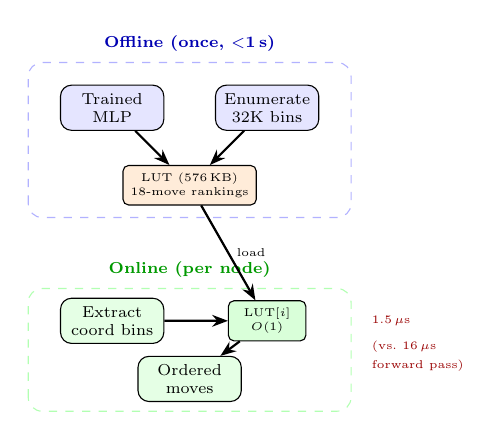
\begin{tikzpicture}[font=\small, scale=0.82, every node/.style={scale=0.82},
  stage/.style={draw, fill=blue!10, rounded corners=4pt, minimum width=1.6cm, minimum height=0.7cm, align=center, font=\scriptsize},
  data/.style={draw, fill=orange!15, rounded corners=2pt, minimum width=1.2cm, minimum height=0.5cm, align=center, font=\tiny},
  arr/.style={-{Stealth[length=2mm]}, thick}
]
  \node[font=\scriptsize\bfseries, text=blue!70!black] at (0, 2.5) {Offline (once, $<$1\,s)};
  \draw[dashed, blue!30, rounded corners=5pt] (-2.5, -0.2) rectangle (2.5, 2.2);
  \node[stage] (train) at (-1.2, 1.5) {Trained\\MLP};
  \node[stage] (enum) at (1.2, 1.5) {Enumerate\\32K bins};
  \node[data] (lut) at (0, 0.3) {LUT (576\,KB)\\18-move rankings};
  \draw[arr] (train) -- (lut);
  \draw[arr] (enum) -- (lut);
  \node[font=\scriptsize\bfseries, text=green!60!black] at (0, -1.0) {Online (per node)};
  \draw[dashed, green!30, rounded corners=5pt] (-2.5, -3.2) rectangle (2.5, -1.3);
  \node[stage, fill=green!10] (coord) at (-1.2, -1.8) {Extract\\coord bins};
  \node[data, fill=green!15] (lookup) at (1.2, -1.8) {LUT[$i$]\\$O(1)$};
  \node[stage, fill=green!10] (order) at (0, -2.7) {Ordered\\moves};
  \draw[arr] (lut) -- (lookup) node[midway, right, font=\tiny] {load};
  \draw[arr] (coord) -- (lookup);
  \draw[arr] (lookup) -- (order);
  \node[font=\tiny, text=red!60!black, anchor=west] at (2.7, -1.8) {1.5\,$\mu$s};
  \node[font=\tiny, text=red!60!black, anchor=west] at (2.7, -2.2) {(vs.\ 16\,$\mu$s};
  \node[font=\tiny, text=red!60!black, anchor=west] at (2.7, -2.5) {forward pass)};
\end{tikzpicture}
\caption{LUT pipeline. \textbf{Offline}: enumerate all 32K coordinate bins, run the MLP once for each, store 18-move rankings (576\,KB). \textbf{Online}: each node does an $O(1)$ array lookup instead of a neural forward pass.}
\label{fig:lut-pipeline}
\end{figure}

\begin{table}[!t]
\centering
\caption{LUT vs.\ per-node neural inference (200 scrambles, seed 42, $K{=}5$).}
\label{tab:lut-benchmark}
\resizebox{\columnwidth}{!}{%
\begin{tabular}{@{}lccccc@{}}
\hline\noalign{\smallskip}
\textbf{Strategy} & \textbf{Solved} & \textbf{Mean} & \textbf{$\leq$20 (\%)} & \textbf{Nodes} & \textbf{Time (ms)} \\
\noalign{\smallskip}\svhline\noalign{\smallskip}
Baseline $K{=}1$ & 200 & 20.77 & 28.0 & 788K & 648 \\
$K{=}5$ none & 200 & 20.35 & 56.0 & 3.39M & 2843 \\
$K{=}5$ + move\_order & 188 & 20.54 & 46.8 & 1.45M & 3374 \\
$K{=}5$ + LUT & 197 & 20.45 & 49.7 & 2.59M & 3047 \\
\noalign{\smallskip}\hline\noalign{\smallskip}
\end{tabular}}
\end{table}

\begin{figure}[!t]
\centering
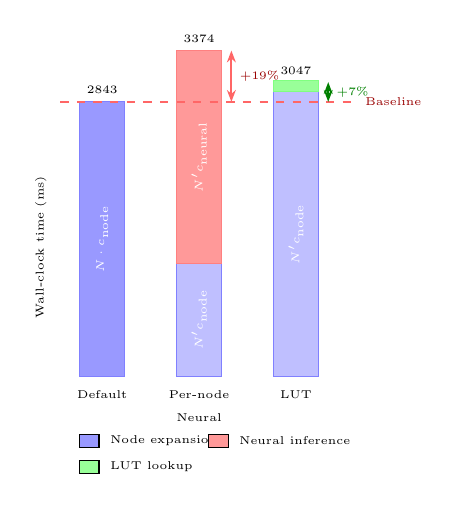
\begin{tikzpicture}[font=\small, scale=0.82, every node/.style={scale=0.82}]
  \def\barw{0.7}
  \def\scale{0.0015}
  \pgfmathsetmacro{\defH}{2843*\scale}
  \draw[fill=blue!40, draw=blue!50] (0, 0) rectangle (\barw, \defH);
  \node[font=\tiny, anchor=south] at (\barw/2, \defH) {2843};
  \node[font=\tiny, below] at (\barw/2, -0.1) {Default};
  \node[font=\tiny, rotate=90, white] at (\barw/2, \defH/2) {$N \cdot c_{\text{node}}$};
  \pgfmathsetmacro{\neuNodeH}{1.21/2.94*2843*\scale}
  \pgfmathsetmacro{\neuInfH}{3374*\scale}
  \draw[fill=blue!25, draw=blue!50] (1.5, 0) rectangle ({1.5+\barw}, \neuNodeH);
  \draw[fill=red!40, draw=red!50] (1.5, \neuNodeH) rectangle ({1.5+\barw}, \neuInfH);
  \node[font=\tiny, anchor=south] at ({1.5+\barw/2}, \neuInfH) {3374};
  \node[font=\tiny, below] at ({1.5+\barw/2}, -0.1) {Per-node};
  \node[font=\tiny, below] at ({1.5+\barw/2}, -0.45) {Neural};
  \node[font=\tiny, rotate=90, white] at ({1.5+\barw/2}, \neuNodeH/2) {$N' c_{\text{node}}$};
  \node[font=\tiny, rotate=90, white] at ({1.5+\barw/2}, {(\neuNodeH+\neuInfH)/2}) {$N' c_{\text{neural}}$};
  \pgfmathsetmacro{\lutH}{3047*\scale}
  \draw[fill=blue!25, draw=blue!50] (3.0, 0) rectangle ({3.0+\barw}, {\lutH - 0.15});
  \draw[fill=green!40, draw=green!50] (3.0, {\lutH - 0.15}) rectangle ({3.0+\barw}, {\lutH + 0.02});
  \node[font=\tiny, anchor=south] at ({3.0+\barw/2}, \lutH) {3047};
  \node[font=\tiny, below] at ({3.0+\barw/2}, -0.1) {LUT};
  \node[font=\tiny, rotate=90, white] at ({3.0+\barw/2}, {(\lutH-0.15)/2}) {$N' c_{\text{node}}$};
  \draw[dashed, red!60, thick] (-0.3, \defH) -- (4.2, \defH);
  \node[font=\tiny, text=red!60!black, anchor=west] at (4.3, \defH) {Baseline};
  \draw[{Stealth[length=1.5mm]}-{Stealth[length=1.5mm]}, thick, red!60] ({1.5+\barw+0.15}, \defH) -- ({1.5+\barw+0.15}, \neuInfH) node[midway, right, font=\tiny, text=red!60!black] {+19\%};
  \draw[{Stealth[length=1.5mm]}-{Stealth[length=1.5mm]}, thick, green!50!black] ({3.0+\barw+0.15}, \defH) -- ({3.0+\barw+0.15}, \lutH) node[midway, right, font=\tiny, text=green!50!black] {$+$7\%};
  \draw[fill=blue!40] (0.0, -1.1) rectangle (0.3, -0.9);
  \node[font=\tiny, anchor=west] at (0.35, -1.0) {Node expansion};
  \draw[fill=red!40] (2.0, -1.1) rectangle (2.3, -0.9);
  \node[font=\tiny, anchor=west] at (2.35, -1.0) {Neural inference};
  \draw[fill=green!40] (0.0, -1.5) rectangle (0.3, -1.3);
  \node[font=\tiny, anchor=west] at (0.35, -1.4) {LUT lookup};
  \node[font=\tiny, rotate=90] at (-0.6, 2.0) {Wall-clock time (ms)};
\end{tikzpicture}
\caption{Inference overhead barrier. Default (2843\,ms): node expansion only. Per-node neural (3374\,ms): 2.4$\times$ fewer nodes but +19\% overhead from inference cost. LUT (3047\,ms): same idea, but $O(1)$ lookup replaces the forward pass, cutting overhead to +7\%.}
\label{fig:overhead-barrier}
\end{figure}

\textbf{Results} (Table~\ref{tab:lut-benchmark}, Fig.~\ref{fig:overhead-barrier}): $K{=}5$ + LUT (3047\,ms) is $1.10\times$ faster than per-node inference (3374\,ms) and within 7\% of the non-neural baseline (2843\,ms), with 98.5\% reliability vs.\ 94.0\% for move\_order. The LUT's node reduction (1.31$\times$) is smaller than full per-node inference (2.34$\times$) because the binned lookup loses fine-grained coordinate information, but the drastically reduced overhead makes the trade-off worthwhile.

\subsection{Hard Cases and Multi-Seed Validation}
\label{sec:hard-cases}

\textbf{Hard cases.} We tested 49 depth-20 scrambles (the superflip timed out under both settings). $K{=}5$ improves $\leq$20-move solutions from 45\% to 71\% at a cost of $71\times$ longer solve time (Table~\ref{tab:hard}, Fig.~\ref{fig:hard-cases}).

\begin{table}[!t]
\centering
\caption{Hard cases: $K{=}1$ vs.\ $K{=}5$ (49 solves, seed 42).}
\label{tab:hard}
\resizebox{\columnwidth}{!}{%
\begin{tabular}{@{}lcccc@{}}
\hline\noalign{\smallskip}
\textbf{Setting} & \textbf{Mean} & \textbf{Median} & \textbf{$\leq$20} & \textbf{Mean ms} \\
\noalign{\smallskip}\svhline\noalign{\smallskip}
$K{=}1$ (baseline) & 20.51 & 21 & 22/49 (45\%) & 435 \\
$K{=}5$ (multi)    & 20.06 & 20 & 35/49 (71\%) & 31133 \\
\noalign{\smallskip}\hline\noalign{\smallskip}
\end{tabular}}
\end{table}

\begin{figure}[!t]
\centering
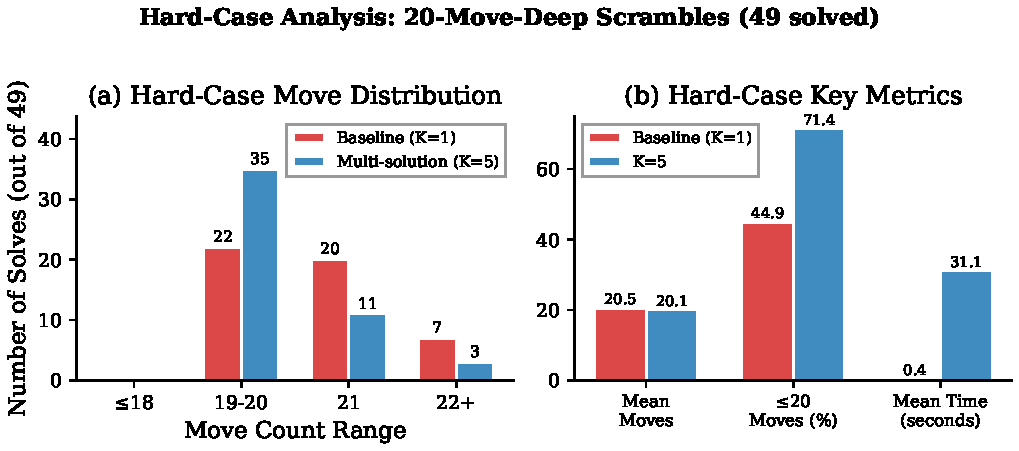
\includegraphics[width=0.85\textwidth]{figures/fig_hard_cases.pdf}
\caption{Hard cases ($K{=}1$ vs.\ $K{=}5$): move distribution and key metrics.}
\label{fig:hard-cases}
\end{figure}

\textbf{Multi-seed validation.} We repeated $K{=}1$ vs.\ $K{=}5$ across four seeds (200 scrambles each). The improvement is consistent: $\Delta = 0.40 \pm 0.09$ moves, with $K{=}5$ $\leq$20 rates of 51.5\%--60.5\% (Table~\ref{tab:multiseed}, Fig.~\ref{fig:multi-seed}). Pooling all 800 pairs: $p < 0.001$, Cohen's $d = 0.59$, 95\% CI $[0.35, 0.45]$.

\begin{table}[!t]
\centering
\caption{Multi-seed validation (200 scrambles each).}
\label{tab:multiseed}
\resizebox{\columnwidth}{!}{%
\begin{tabular}{@{}lcccc@{}}
\hline\noalign{\smallskip}
\textbf{Seed} & \textbf{BL Mean} & \textbf{K5 Mean} & \textbf{$\Delta$} & \textbf{K5 $\leq$20 (\%)} \\
\noalign{\smallskip}\svhline\noalign{\smallskip}
42  & 20.77 & 20.30 & 0.47 & 60.5 \\
123 & 20.85 & 20.36 & 0.49 & 57.5 \\
456 & 20.67 & 20.31 & 0.36 & 57.0 \\
789 & 20.74 & 20.45 & 0.29 & 51.5 \\
\noalign{\smallskip}\svhline\noalign{\smallskip}
\textbf{Mean $\pm$ SD} & $20.75 \pm 0.07$ & $20.35 \pm 0.07$ & $0.40 \pm 0.09$ & $56.6 \pm 3.8$ \\
\noalign{\smallskip}\hline\noalign{\smallskip}
\end{tabular}}
\end{table}

\begin{figure}[!t]
\centering
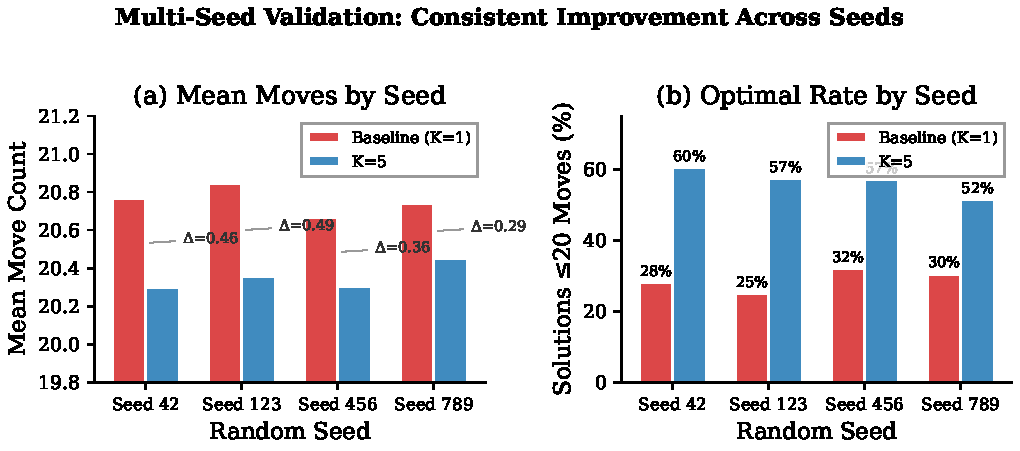
\includegraphics[width=0.85\textwidth]{figures/fig_multi_seed.pdf}
\caption{Multi-seed validation. $K{=}5$ consistently outperforms the baseline across all four seeds, roughly doubling the $\leq$20-move rate.}
\label{fig:multi-seed}
\end{figure}

%==============================================================================
\section{Discussion}
\label{sec:discussion}
%==============================================================================

\subsection{Why Multi-Solution Search Works}

Different Phase~1 solutions reach different points in $G_1$, and the Phase~2 distance back to the identity varies. The first Phase~1 solution is essentially random among those at the minimum depth; trying $K$ of them and keeping the best is like taking the minimum of $K$ draws from the Phase~2 length distribution.

The diminishing returns beyond $K{=}3$ indicate that Phase~2 lengths have limited variance: most endpoints lead to similarly long Phase~2 solutions, so additional samples have decreasing marginal value. Under the 5\,s timeout, $K{=}10$ and $K{=}5$ produce identical results---the solver exhausts available Phase~1 endpoints regardless.

\subsection{Three Levels of Neural Failure---and How We Fixed Two}

Our investigation reveals a layered explanation:

\textbf{Level 1: Low accuracy.} With scalar features (9~dims), the predictor achieves 5.6\%---random among 18 moves. This is the immediate cause of failure.

\textbf{Level 2: Representation bottleneck (resolved).} Switching to 161-dimensional binned features raises accuracy to 83.3\%. The bottleneck was the input, not the model: the same MLP architecture suffices when given structurally informative inputs. Binned encoding preserves the discrete group-theoretic structure that scalar normalisation destroys.

\textbf{Level 3: Inference overhead barrier (largely resolved).} Even with 83.3\% accuracy and $2.4\times$ node reduction, per-node inference in Python is too expensive (Eq.~\ref{eq:overhead}). Architecture scaling makes this \emph{worse} (Table~\ref{tab:arch-comparison}). LUT precomputation largely \emph{eliminates} it: per-node cost drops from $\sim$16\,$\mu$s to $\sim$1.5\,$\mu$s, and overhead drops from $+19\%$ to $+7\%$ of the non-neural baseline.

\textbf{Bottom line.} The overhead barrier is an engineering constraint, not a fundamental limit. Compiled C/CUDA inference or finer-grained LUTs would further close the remaining gap.

\subsection{Comparison with DeepCubeA}

DeepCubeA~\cite{deepcubea} uses a much larger ResNet ($\sim$500K parameters), trains for 2~days on GPUs with millions of samples, and uses weighted~A* that expands far fewer nodes ($\sim$1K vs.\ our $\sim$1M). This makes per-node neural cost less critical for DeepCubeA. Our work shows that with the right feature representation, even a tiny MLP can achieve high prediction accuracy (83.3\%), and that \emph{input representation matters more than model scale} for this domain.

\subsection{Deployment Recommendations}

\begin{table}[!t]
\centering
\caption{Recommended settings for different use cases.}
\label{tab:deployment-summary}
\resizebox{\columnwidth}{!}{%
\begin{tabular}{@{}llcc@{}}
\hline\noalign{\smallskip}
\textbf{Scenario} & \textbf{Setting} & \textbf{Mean ms} & \textbf{Mean moves} \\
\noalign{\smallskip}\svhline\noalign{\smallskip}
C backend (fastest) & $K{=}1$, no budget  & 11.8  & 20.77 \\
Real-time (Python)  & $K{=}1$, no budget  & 648   & 20.77 \\
Balanced            & $K{=}3$, no budget  & 2814  & 20.36 \\
Best quality        & $K{=}5$, no budget  & 2843  & 20.35 \\
Neural + LUT        & $K{=}5$ + LUT       & 3047  & 20.45 \\
\noalign{\smallskip}\hline\noalign{\smallskip}
\end{tabular}}
\end{table}

For most applications, $K{=}3$ offers the best trade-off (Table~\ref{tab:deployment-summary}): 98\% of the quality gain at 99\% of the cost. The C backend makes even $K{=}5$ fast enough for real-time use ($<$50\,ms).

%==============================================================================
\section{Conclusion}
\label{sec:conclusion}
%==============================================================================

We extended Kociemba's Two-Phase Algorithm with multi-solution search, neural move ordering, and formal analysis. Our main findings:

\begin{enumerate}[leftmargin=*]
  \item \textbf{Multi-solution search works.} $K{=}5$ reduces mean moves by 0.42 ($p < 0.001$, $d = 0.70$) and doubles $\leq$20-move solutions (28\%$\to$56\%), robust across four seeds.
  \item \textbf{Representation is the bottleneck, not model size.} Binned coordinate features (161~dims) raise accuracy from 5.6\% to 83.3\% and yield $2.4\times$ node reduction.
  \item \textbf{Inference overhead is real but solvable.} Per-node neural inference negates the node savings in Python. LUT precomputation (32K entries, 576\,KB) largely eliminates this overhead ($+7\%$ vs.\ $+19\%$).
  \item \textbf{Na\"ive neural bounds are harmful.} Using neural predictions as IDA* lower bounds causes exponential blowup (Theorem~\ref{thm:bound-paradox}). The correct integration is move ordering.
\end{enumerate}

\textbf{Future work.} Incorporating Phase~2 coordinates into the LUT, using graph neural networks on the cubie adjacency structure, and parallelising Phase~1 search across multiple cores are all promising directions. We particularly recommend Phase~1 endpoint prediction---learning which $G_1$ states lead to short Phase~2 solutions---as a way to make multi-solution search smarter rather than just broader.

\textbf{Reproducibility.} All benchmarks are reproducible via: \texttt{python benchmark.py --scrambles 200 --compare-baseline --max-phase1 5 --seed 42 -v}. Results, models, and scripts are provided.

%==============================================================================
\begin{thebibliography}{99.}
\bibitem{kociemba}
H.\,Kociemba, ``Two-Phase Algorithm,'' [Online]. Available:
\url{https://kociemba.org/cube.htm}.

\bibitem{godnumber}
T.\,Rokicki, H.\,Kociemba, M.\,Davidson, and J.\,Dethridge,
``God's Number is 20,'' 2010. [Online]. Available:
\url{http://www.cube20.org/}.

\bibitem{muodov}
muodov/kociemba, ``Python package: C and Python implementations of
Kociemba's two-phase algorithm,'' [Online]. Available:
\url{https://github.com/muodov/kociemba}.

\bibitem{deepcubea}
F.\,Agostinelli, S.\,McAleer, A.\,Shmakov, and P.\,Baldi,
``Solving the {R}ubik's {C}ube with Deep Reinforcement Learning and
Search,'' \textit{Nature Mach.\ Intell.}, vol.\,1, pp.\,356--363, 2019.

\bibitem{korf1997}
R.\,E.\,Korf, ``Finding Optimal Solutions to {R}ubik's {C}ube Using
Pattern Databases,'' in \textit{Proc.\ AAAI Conf.\ Artif.\ Intell.},
1997, pp.\,700--705.

\bibitem{thistlethwaite1981}
M.\,Thistlethwaite, ``A 45-Move Algorithm for {R}ubik's {C}ube,''
unpublished manuscript, 1981.

\bibitem{brunetto2017}
R.\,Brunetto and O.\,Trunda, ``Deep Heuristic-Learning in the
{R}ubik's {C}ube Domain: An Experimental Evaluation,''
\textit{Proc.\ ITAT}, pp.\,57--64, 2017.

\bibitem{shen2020}
W.\,Shen, F.\,Trevizan, and S.\,Thi\'ebaux, ``Learning
Domain-Independent Heuristics for Grounded and Lifted Planning,''
in \textit{Proc.\ AAAI Conf.\ Artif.\ Intell.}, 2020,
pp.\,9883--9891.

\bibitem{ferber2022}
P.\,Ferber, F.\,Geissmann, T.\,Helmert, \textit{et al.},
``Neural Network Heuristics for Classical Planning: A Study of
Hyperparameter Space,'' in \textit{Proc.\ Eur.\ Conf.\ Artif.\
Intell.\ (ECAI)}, 2022, pp.\,839--846.

\bibitem{felner2004}
A.\,Felner, R.\,E.\,Korf, and S.\,Hanan,
``Additive Pattern Database Heuristics,'' \textit{J.\ Artif.\
Intell.\ Res.\ (JAIR)}, vol.\,22, pp.\,279--318, 2004.

\bibitem{fridrich}
J.\,Fridrich, ``CFOP Method,'' [Online]. Available:
\url{https://www.speedsolving.com/wiki/index.php/CFOP_method}.

\bibitem{korf1985}
R.\,E.\,Korf, ``Depth-First Iterative-Deepening: An Optimal
Admissible Tree Search,'' \textit{Artif.\ Intell.}, vol.\,27,
no.\,1, pp.\,97--109, 1985.

\bibitem{hart1968}
P.\,E.\,Hart, N.\,J.\,Nilsson, and B.\,Raphael, ``A Formal Basis
for the Heuristic Determination of Minimum Cost Paths,''
\textit{IEEE Trans.\ Syst.\ Sci.\ Cybern.}, vol.\,4, no.\,2,
pp.\,100--107, 1968.

\bibitem{pearl1984}
J.\,Pearl, \textit{Heuristics: Intelligent Search Strategies for
Computer Problem Solving}.\quad Reading, MA: Addison-Wesley, 1984.

\bibitem{culberson1998}
J.\,C.\,Culberson and J.\,Schaeffer, ``Pattern Databases,''
\textit{Comput.\ Intell.}, vol.\,14, no.\,3, pp.\,318--334, 1998.

\bibitem{korf2002}
R.\,E.\,Korf and A.\,Felner, ``Disjoint Pattern Database
Heuristics,'' \textit{Artif.\ Intell.}, vol.\,134, no.\,1--2,
pp.\,9--22, 2002.

\bibitem{silver2016}
D.\,Silver \textit{et al.}, ``Mastering the Game of {G}o with Deep
Neural Networks and Tree Search,'' \textit{Nature}, vol.\,529,
pp.\,484--489, 2016.

\bibitem{silver2017}
D.\,Silver \textit{et al.}, ``Mastering the Game of {G}o Without
Human Knowledge,'' \textit{Nature}, vol.\,550, pp.\,354--359, 2017.

\bibitem{arfaee2011}
S.\,J.\,Arfaee, S.\,Zilles, and R.\,C.\,Holte, ``Learning
Heuristic Functions for Large State Spaces,'' \textit{Artif.\
Intell.}, vol.\,175, no.\,16--17, pp.\,2075--2098, 2011.

\bibitem{schaeffer1989}
J.\,Schaeffer, ``The History Heuristic and Alpha-Beta Search
Enhancements in Practice,'' \textit{IEEE Trans.\ Pattern Anal.\
Mach.\ Intell.}, vol.\,11, no.\,11, pp.\,1203--1212, 1989.

\bibitem{reinefeld1994}
A.\,Reinefeld and T.\,A.\,Marsland, ``Enhanced Iterative-Deepening
Search,'' \textit{IEEE Trans.\ Pattern Anal.\ Mach.\ Intell.},
vol.\,16, no.\,7, pp.\,701--710, 1994.

\bibitem{joyner2008}
D.\,Joyner, \textit{Adventures in Group Theory: {R}ubik's {C}ube,
{M}erlin's Machine, and Other Mathematical Toys}, 2nd\,ed.\quad
Baltimore, MD: Johns Hopkins Univ.\ Press, 2008.

\bibitem{cohen1988}
J.\,Cohen, \textit{Statistical Power Analysis for the Behavioral
Sciences}, 2nd\,ed.\quad Hillsdale, NJ: Lawrence Erlbaum, 1988.

\bibitem{efron1993}
B.\,Efron and R.\,J.\,Tibshirani, \textit{An Introduction to the
Bootstrap}.\quad New York: Chapman and Hall/CRC, 1993.

\bibitem{david2003}
H.\,A.\,David and H.\,N.\,Nagaraja, \textit{Order Statistics},
3rd\,ed.\quad Hoboken, NJ: Wiley, 2003.

\bibitem{hinton2015}
G.\,Hinton, O.\,Vinyals, and J.\,Dean, ``Distilling the Knowledge
in a Neural Network,'' in \textit{Proc.\ NeurIPS Deep Learn.\
Workshop}, 2015.

\bibitem{kingma2015}
D.\,P.\,Kingma and J.\,Ba, ``{A}dam: A Method for Stochastic
Optimization,'' in \textit{Proc.\ Int.\ Conf.\ Learn.\ Represent.\
(ICLR)}, 2015.

\bibitem{demaine2018}
E.\,D.\,Demaine, M.\,L.\,Demaine, S.\,Eisenstat, A.\,Lubiw, and
A.\,Winslow, ``Algorithms for Solving {R}ubik's {C}ubes,'' in
\textit{Proc.\ Eur.\ Symp.\ Algorithms (ESA)}, 2011,
pp.\,689--700.

\bibitem{paszke2019}
A.\,Paszke \textit{et al.}, ``{P}y{T}orch: An Imperative Style,
High-Performance Deep Learning Library,'' in \textit{Advances in
Neural Inf.\ Process.\ Syst.\ (NeurIPS)}, vol.\,32, 2019.

\end{thebibliography}

\end{document}
